%-*- coding: UTF-8 -*-
% notes.tex
%
\documentclass[UTF8]{article}
\usepackage{geometry}
\geometry{a4paper, centering, scale=0.8}
\usepackage{minted}
\usepackage{hyperref}
\usepackage{indentfirst}    % to indent the first paragraph of a section
\usepackage{graphicx}       % to insert figures
\usepackage{amsmath}        % to type some math equations
\usepackage{amssymb}        % to use some special math font
\usepackage{IEEEtrantools}  % to use IEEEeqnarray
\usepackage{algorithm2e}    % to use algorithm environment
\usepackage{multicol}       % to display some content in multi-columns
\setlength{\columnseprule}{0.4pt}   % set the rule's width of multicols
\setlength{\columnsep}{5em}         % set the sep of multicols

% Math notation
% refered to https://github.com/exacity/deeplearningbook-chinese/blob/master/math_symbol.tex
\newcommand{\Scalar}[1]{\mathit{#1}}                % Scalar, the default math font
\newcommand{\Vector}[1]{\boldsymbol{\mathit{#1}}}   % Vector
\newcommand{\Matrix}[1]{\boldsymbol{\mathit{#1}}}   % Matrix
\newcommand{\Tensor}[1]{\textsf{\textbf{#1}}}       % Tensor
\newcommand{\Set}[1]{\mathbb{#1}}                   % Set
\newcommand{\Cal}[1]{\mathcal{#1}}                  % Math Cal

% Draw the lines in a matrix, which is composed by a series of vectors
\newcommand{\vRule}{\rule{0.3pt}{10mm}}             % vertical rule
\newcommand{\hRule}{\,\rule[1mm]{10mm}{0.3pt}\,}    % horizontal rule

\title{Deep Learning Specialization \\
        Improving Deep Neural Networks: Hyperparameter tuning, Regularization and Optimization \\
        Learning Notes}
\author{Du Ang \\ \texttt{du2ang233@gmail.com} }
\date{\today}

\begin{document}
\maketitle

\tableofcontents
\newpage

\section{Practical aspects of Deep Learning}
\subsection{Setting up your Machine Learning Application}
\subsubsection{Train/Dev/Test sets}
When training a neural network, you have to make a lot of decisions, such as choosing the number of
layers of the neural network, choosing the number of hidden units of each hidden layer, choosing
the learning rates and activations.

Applied machine learning is a highly iterative process. At first, you have some ideas and make some
decisions. Then you implement the ideas with code in programming. You run some experiments and you
get back a result that tells you how well this particular network, or this particular configuration
works. And based on the outcome, you might refine your ideas and change your choices and maybe keep
iterating in order to try to find a better and beter neural network.

Intuitions from one domain or from one application area often do not transfer to other application
areas. And the best choices may depend on the amount of data you have, the number of input features
you have through your computer configuration and whether you're training on GPUs or CPUs. Even very
experienced deep learning people find it almost impossible to correctly guess the best choice of
hyperparameters the very first time. And so today, applied deep learning is a very iterative
process where you just have to go around this cycle many times to hopefully find a good choice of
network for your application. So one of the things that determine how quickly you can make progress
is how efficiently you can go around this cycle.

Setting up your data sets well in terms of your train, development and test sets can make you much
more efficient at that. The dataset can be separated into three parts: training set, dev set
(development set, hold-out cross validation) and test set.

In the previous era of machine learning, it was common practice to take all your data and split it
accordin to 70/30 percent in terms of a people often talk about the 70/30 train test splits, if you
don't have an explicit dev set. Or maybe a 60/20/20 percent split in terms of 60\% train, 20\% dev
and 20\% test. And several years ago, this was the widely considered as the best practice in
machine learning, if you have 100, 1000 or 10,000 examples.

But in modern big data era, where you might have a million examples in total, then the trend is
that your dev and test sets have been becoming a much smaller percentage of the total. Because
remember, the goal of the dev set is that you're going to test different algorithms on it and see
which algorithm choices works better. So the dev set just needs to to be big enough for you to
evaluate, for example, two different algorithm choices or ten different algorithm choices and
quickly decide which one is doing better. And you might not need a whole 20\% of your data for that.
Similarly, the main goal of your test set is, given your final classifier, to give you a pretty
confident estimate of how well it's doing.

\begin{description}
    \item[Previous era (small exampels): ] training set/dev set/test set : 60/20/20
    \item[Big data era: ] training set/dev set/test set : 98/1/1
\end{description}

One other trend we're seeing in the era of modern deep learning is that more and more people train
on mismatched train and test distributions. Let's say you're building an app that lets users upload
a lot of pictures and your goal is to find pictures of cats in order to show your users. Maybe all
your training set comes from cat pictures downloaded off the Internet, but your dev and test sets
might comprise cat pictures from user using our app. It turns out that a lot of webpages have very
high resolution, very professional, very nicely framed pictures of cats. But maybe your users are
uploading blurrier, lower resolution images just taken with a cell phone camera in a more casual
condition. And so the two distributions of data may be different. The rule of thumb to follow in
this case is to make sure that the dev and test sets come from the same distribution.

Finally, it might be okay to not have a test set. If you have only a dev set but not a test set,
what you do is you train on the training set and then try different model architectures. Evaluate
them on the dev set, and then use that to iterate and try to get to a good model. Because you've
fit your data to the dev set, this no longer gives you an unbiased estimate of performance.

In machine learning world, when you have just a train and a dev set but no separate test set, most
people will call this a training set and they will call the dev set the test set. But what they
actually end up doing is using the test as a hold-out cross validation set. Which maybe isn't
complete a great use of terminology, because they're overfitting to the test set.

Having set up a train dev and test set will allow you to integrate more quickly. It will also allow
you to more efficently measure the bias and variance of your algorithm, so you can more efficiently
select ways to improve your algorithm.

\subsubsection{Bias/Variance}
\begin{figure}[htb]
    \centering
    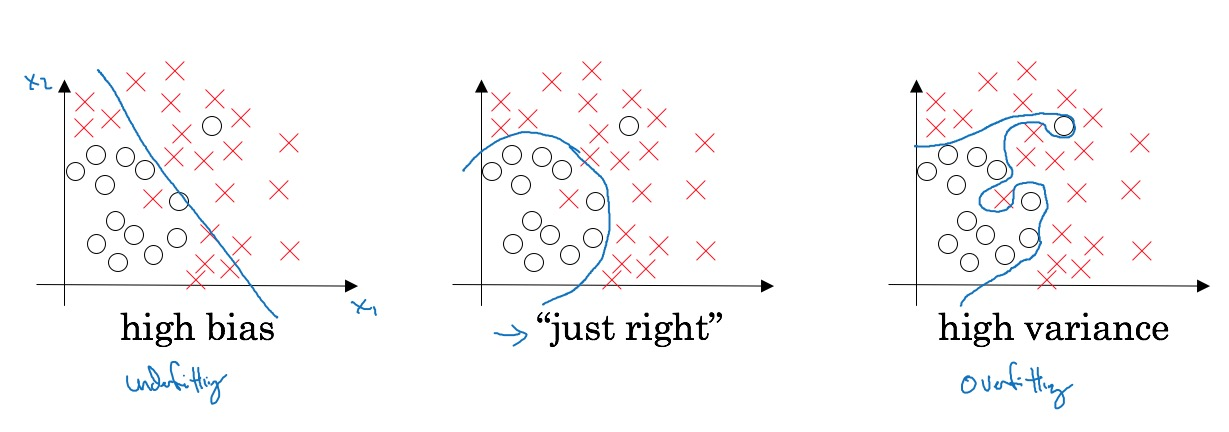
\includegraphics[width=40em]{figures/bias-and-variance-1}
    \caption{Decision boundaries of different classifier on 2D examples}
\end{figure}

\begin{figure}[htb]
    \centering
    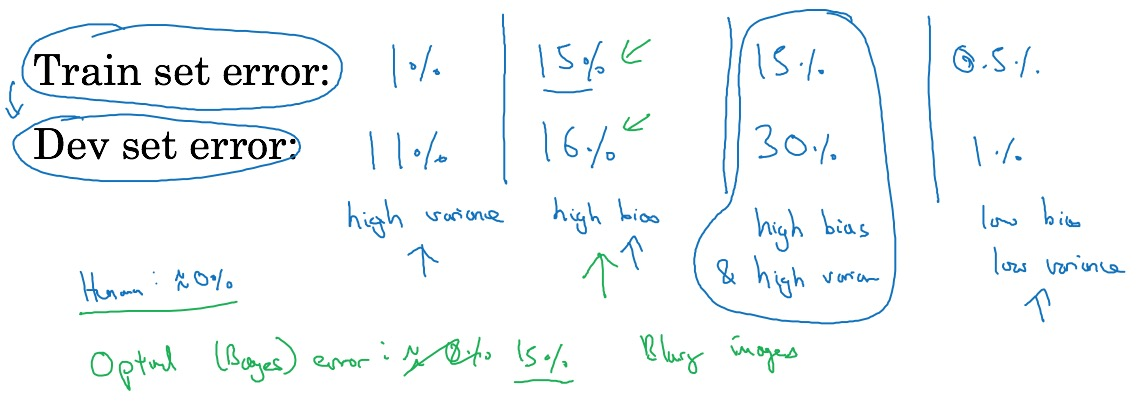
\includegraphics[width=40em]{figures/bias-and-variance-2}
    \caption{Bias or Variance showed by training set error and dev set error. It is related to the
    optimal error (base error), which is determined by the common practices and our expectation.}
\end{figure}

\begin{figure}[htb]
    \centering
    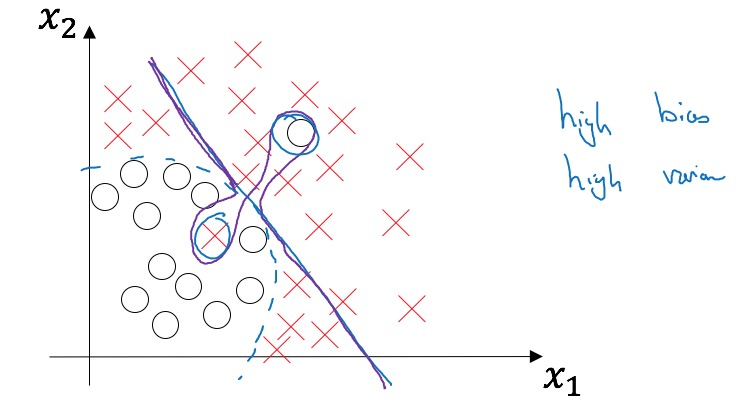
\includegraphics[width=30em]{figures/bias-and-variance-3}
    \caption{The purple decision boundary shows a high bias and high variance case}
\end{figure}

\subsubsection{Basic Recipe for Machine Learning}
\begin{figure}[htb]
    \centering
    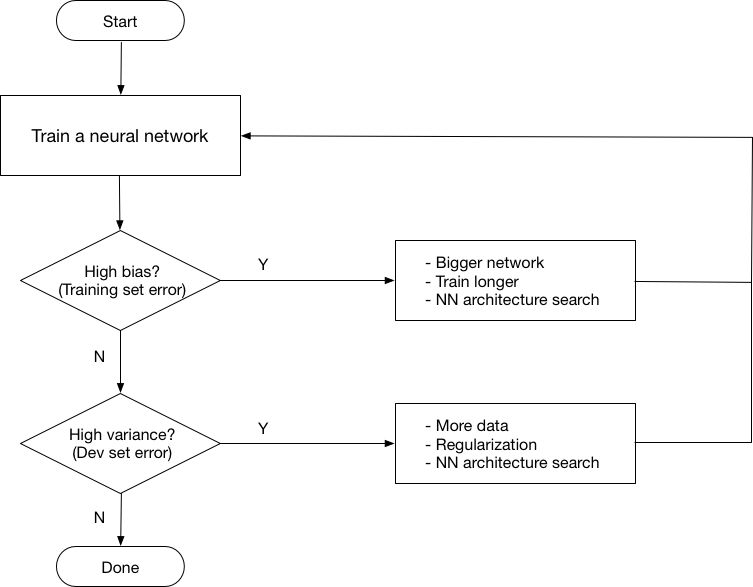
\includegraphics[width=30em]{figures/machine-learning-recipe}
    \caption{Basic recipe for Machine Learning}
    \label{fig:machine-learning-recipe}
\end{figure}

Whereas getting a bigger network almost always helps, and training longer doesn't always help, but
it certainly never hurts. Usually if you have a big enough network, you should usually fit the
training data well so long as it's problem that is possible for someone to do.

If you have high variance problem, the best way to solve high variance problem is to get more data.
But sometimes you can't get more data, or you could try regularization to reduce overfitting. But
if you can find a more appropriate neural network architecture, sometimes that can reduce your
variance problem as well, as well as reduce your bias problem.

Like Figure~\ref{fig:machine-learning-recipe} shows, there are a couple of points to notice. First
is that, depending on whether you have high bias or high variance, the set of things hou should try
could be quite different. So usually use the training dev set to try to diagnose if you have a bias
or variance problem, and then use that to select the appropriate subset of things to try. So for
example, if you actually have a high bias problem, getting more training data is actually not going
to help. Or at least it's not the most efficient thing to do.

\paragraph{Bias variance trade-off} In the earlier era of machine learning, there used to be a lot
of discussion on what is called the bias variance trade-off. And the reason for that was that, for
a lot of the things you could try, you could increase bias and reduce variance, or reduce bias and
increase variance. Back in the pre-deep learning era, we didn't have many tools, we didn't have
as many that just reduce bias or that just reduce variance without hurting the other one. But in
the modern deep learning, big data era, so long as you can keep training a bigger network, and so
long as you can keep getting more data, which isn't always just reduces your bias without
necessarily hurting your variance, so long as you regularize appropriately. And getting more data
always reduces your variance and doesn't hurt your bias much. So what's really happened is that,
with these two steps, the ability to train, pick a network, or get more data, we now have tools to
drive down variance, without really hurting the other thing that much.

\subsection{Regularizing your neural network}
\subsubsection{Regularization}
If you suspect your neural network is overfitting your data, that is you have a high variance
problem, one of the first thing you should try is probably regularization. The other way to address
high variance is to get more training data, which is also quite reliable, but you can't always get
more training data, or it could be more expensive to get more data. But adding regularization
will often help to prevent overfitting, or to reduce the errors in your network.

\paragraph{Logistic regression}
$$ \underset{\Vector{w}, b}{\text{min}} J(\Vector{w}, b) \qquad
\Vector{w} \in \Set{R}^{n_x}, b \in \Set{R} $$
$$ J(\Vector{w}, b) = \frac{1}{m} \sum_{i=1}^m \Cal{L}(\hat{y}^{(i)}, y^{(i)})
+ \frac{\lambda}{2m} ||\Vector{w}||_2^2 $$

\begin{description}
    \item[$L_2$ Norm (squared)]
    $\displaystyle ||\Vector{w}||_2^2 = \sum_{j=1}^{n_x} \Vector{w}_j^2 = \Vector{w}^T \Vector{w} $
    \item[$L_1$ Norm]
    $\displaystyle ||\Vector{w}||_1 = \sum_{j=1}^{n_x}|\Vector{w}_j| $ \qquad
    (Using $L_1$ Norm will make $\Vector{w}$ sparse)
\end{description}

The $\lambda$ means ``regularization parameter'', it helps prevent overfitting. In Python,
\mintinline{python}{lambda} is a reserved keyword, so we use \texttt{lambd}, without \texttt{a}, to
represent the lambda regulzarization parameter.

\paragraph{Neural network}
$$ J(\Matrix{W^{[1]}}, \Vector{b^{[1]}}, \ldots, \Matrix{W}^{[L]}, \Vector{b}^{[L]})
= \frac{1}{m} \sum_{i=1}^{m} \Cal{L}(\hat{\Vector{y}}^{(i)}, \Vector{y}^{(i)})
+ \frac{\lambda}{2m} \sum_{l=1}^L ||\Matrix{W}^{[l]}||_F^2 \qquad
\Matrix{W} \in \Set{R}^{(n^{[l]}, n^{[l-1]})}$$

\begin{description}
    \item[Frobenius Norm (squared)]
    $ \displaystyle ||\Matrix{W}^{[l]}||_F^2 = \sum_{i=1}^{n^{[l-1]}} \sum_{j=1}^{n^{[l]}}
    (\Matrix{W}_{ij})^2 $ \\ (the sum of squares of elements of a matrix, just like $L_2$ norm)
\end{description}

In backpropagation,
$$ \text{d}\Matrix{W}^{[l]} = \frac{1}{m} \text{d}\Matrix{Z}^{[l]} {\Matrix{A}^{[l-1]}}^T
+ \frac{\lambda}{m} \Matrix{W}^{[l]} $$
$$ \Matrix{W}^{[l]} := \Matrix{W}^{[l]} - \alpha \text{d}\Matrix{W}^{[l]} $$

$L_2$ norm sometimes is called ``weight decay'', that's because
\begin{IEEEeqnarray*}{rCl}
\Matrix{W}^{[l]} := \Matrix{W}^{[l]} - \alpha \text{d}\Matrix{W}^{[l]}
= \Matrix{W}^{[l]} - \alpha (\frac{1}{m} \text{d}\Matrix{Z}^{[l]} {\Matrix{A}^{[l-1]}}^T
+ \frac{\lambda}{m} \Matrix{W}^{[l]})
= (1 - \frac{\alpha \lambda}{m}) \Matrix{W}^{[l]}
- \frac{\alpha}{m} \text{d}\Matrix{Z}^{[l]}{\Matrix{A}^{[l-1]}}^T
\end{IEEEeqnarray*}












\end{document}
